\documentclass[10pt]{article}

% ---------------------------------------------------------------- layout (NeurIPS-style page geometry)
\usepackage[letterpaper,textwidth=5.5in,textheight=9in,top=1in,headheight=12pt,headsep=25pt,footskip=30pt]{geometry}
\usepackage[T1]{fontenc}
\usepackage{times}
\usepackage[utf8]{inputenc}
\usepackage{amsmath,amssymb}
\usepackage{booktabs,multirow,array}
\usepackage{graphicx}
\usepackage{xcolor}
\usepackage[numbers,sort&compress]{natbib}
\usepackage[hidelinks]{hyperref}
\usepackage{microtype}
\usepackage{caption,subcaption}
\usepackage{tikz}
\usetikzlibrary{positioning,arrows.meta,fit,calc}
\usepackage{titlesec}
\usepackage{enumitem}

\captionsetup{font=small,labelfont=bf}
\titleformat{\section}{\large\bfseries}{\thesection}{1em}{}
\titleformat{\subsection}{\normalsize\bfseries}{\thesubsection}{1em}{}
\titleformat{\paragraph}[runin]{\normalsize\bfseries}{}{}{}[.]
\setlength{\parindent}{0pt}
\setlength{\parskip}{5.5pt}
\setlist{itemsep=1pt,topsep=2pt}
\titlespacing*{\paragraph}{0pt}{4pt}{0.6em}
\titlespacing*{\subsection}{0pt}{8pt}{3pt}
\emergencystretch=1.5em
\definecolor{cres}{HTML}{2A78D6}
\definecolor{cafno}{HTML}{EB6834}
\definecolor{cgray}{HTML}{6B6B66}
\newcommand{\PM}{PM\textsubscript{2.5}}

\makeatletter
\renewcommand{\@maketitle}{%
  \vbox{\hsize\textwidth\linewidth\hsize\vskip 0.1in
    \hrule height 4pt\vskip 0.25in
    \centering{\LARGE\bfseries\@title\par}\vskip 0.29in
    \hrule height 1pt\vskip 0.09in
    \centering\@author\par\vskip 0.3in}}
\makeatother

\title{Pipeline Before Backbone: A Controlled Comparison of Fourier Neural Operators and Convolutional-Recurrent Networks for 16-Hour \PM{} Forecasting over India}

\author{%
  \begin{tabular}{c}
  Vetriselvan R, Hrishi Dongre, Pampana Sree Adithya, Ishan Goyal, Vedant Madne \\[2pt]
  \small Team T024, Section A - DL Project 19: Air quality forecasting via gradient boosting and LSTM models
  \end{tabular}}

\begin{document}
\maketitle

\begin{center}\textbf{\large Abstract}\end{center}
\vspace{-4pt}
\begin{quote}
Country-scale \PM{} forecasts from chemical transport models such as WRF-Chem are expensive to run, which motivates learned emulators. We study 16-hour \PM{} forecasting on a $140\times124$ grid (about 25\,km) over India from 10 hours of WRF-Chem fields, and ask a simple question that the literature rarely isolates: how much of a forecaster's skill comes from the network architecture, and how much from the pipeline around it? Over eight development iterations we built a physics-informed pipeline: ventilation, advection and tendency channels, a log-space persistence residual, a leak-free temporal validation that reproduces the test conditions, a loss aligned with the evaluation metric, and seed ensembles with per-horizon calibration. It raised the held-out test score from 0.8218 to 0.8914. We then ran a controlled study in which five architectures were trained inside this one fixed pipeline, with decision rules fixed before each stage and 1, 2 and 5 seeds. A U-Net with a convolutional GRU over lead time (ResGRU-UNet) beats an Adaptive Fourier Neural Operator hybrid (AFNO V4) on all 25 seed pairs, at every lead hour, in every validation month and in 95\% of grid cells, and also on MAE (6.32 vs 6.99\,$\mu$g\,m$^{-3}$), RMSE (18.04 vs 19.45) and $R^2$ (0.892 vs 0.874). Yet moving the same network into the improved pipeline gained 6 to 8 times more than swapping the network. We further show that model rankings depend on the metric, that calibration trades regression error for the benchmark score, and that the Fourier model shows a larger generalization gap that none of four single-change ablations removes.
\end{quote}

% ================================================================
\section{Introduction}

Fine particulate matter (\PM) is the leading environmental health risk in India: air pollution was associated with an estimated 1.67 million deaths there in 2019 \citep{pandey2021}. Reliable country-wide forecasts a day ahead support warnings and interventions, but they usually come from online chemistry-transport models such as WRF-Chem \citep{grell2005}, which couple meteorology, emissions, chemistry and transport and are costly to run at high resolution. Learned emulators that map recent simulated states to future \PM{} fields could make such forecasts cheap.

Two families of architectures are natural candidates. Fourier neural operators \citep{li2021fno} and their adaptive variant AFNO \citep{guibas2022afno} mix information globally in the spectral domain and underpin data-driven weather models such as FourCastNet \citep{pathak2022fourcastnet}. Convolutional-recurrent networks, from ConvLSTM \citep{shi2015convlstm} to ConvGRU \citep{ballas2016convgru} and U-Net hybrids \citep{ronneberger2015unet,leinonen2021}, propagate local information step by step. Reported comparisons between such families usually differ in more than the network: inputs, validation design, loss, post-processing and training budget change together, so an observed difference cannot be credited to the architecture.

This paper reports a complete development history on one dataset, followed by a controlled comparison. Our contributions are:
\begin{itemize}[leftmargin=14pt]
\item A physics-informed, leak-free forecasting pipeline, developed over eight iterations, with the reason for each change and its measured effect (Section~\ref{sec:pipeline}). Its main elements are physically motivated input channels, a log-space persistence residual, a temporal hold-out that reproduces the test conditions, a metric-aligned loss, and ensembling with per-horizon calibration.
\item A controlled backbone study: five architectures in one fixed pipeline, with decision rules written down before each stage, and 1, 2 and 5 seeds with block-bootstrap intervals (Section~\ref{sec:study}). ResGRU-UNet is better than AFNO V4 on every seed pair and every metric we report.
\item Evidence that the pipeline mattered more than the backbone: the same network gained +0.0292 in held-out test score from the pipeline, against a +0.0036 backbone gap at the same setting.
\item Analyses that matter for practice (Sections~\ref{sec:analysis} and \ref{sec:why}): regression metrics for every model and three baselines including ridge regression, metric-dependent model rankings, a calibration trade-off, spatial error maps, and ablations together with a generalization gap of the Fourier model.
\end{itemize}

% ================================================================
\section{Related work}

\paragraph{Neural operators}
The Fourier Neural Operator learns mappings between function spaces through spectral convolutions \citep{li2021fno}. AFNO replaces the per-mode weights with a block-diagonal MLP over Fourier modes with soft-thresholding, as an efficient token mixer \citep{guibas2022afno}, and powers FourCastNet's global forecasts \citep{pathak2022fourcastnet}. AdaptFNO adds adaptive modes and multiscale learning for climate fields \citep{dang2025adaptfno}. For Indian air quality, CoNOAir, a complex neural operator, is reported to outperform FNO for carbon monoxide forecasting in Indian cities \citep{bedi2025conoair}.

\paragraph{Spatiotemporal prediction}
ConvLSTM introduced convolutional recurrence for precipitation nowcasting \citep{shi2015convlstm}, followed by TrajGRU \citep{shi2017trajgru}; ConvGRU is the gated-recurrent counterpart \citep{ballas2016convgru}. SimVP showed that a purely convolutional encoder, translator and decoder can match recurrent models \citep{gao2022simvp}. Shortcut recurrent-convolutional networks with U-Net-like skips were used for weather prediction \citep{leinonen2021}. For particulate matter over the Indian subcontinent, lightweight deep learning models were reported to outperform the Aurora foundation model at short horizons \citep{kushwaha2025}.

\paragraph{Evaluation}
We use the symmetric mean absolute percentage error, whose asymmetry in additive error is well known \citep{goodwin1999}, standard regression metrics, and naive and seasonal-naive baselines \citep{hyndman2021}. For dependent data, blocked rather than random validation is necessary \citep{roberts2017}.

% ================================================================
\section{Data, task and evaluation}
\label{sec:data}

\paragraph{Data}
We use the WRF-Chem simulation dataset released by the organizers of the ANRF AISEHack 2026 (Theme 2, IIT Delhi) on Kaggle \citep{aisehack2026}. Training data cover four months of 2016 that represent the seasons (April, July, October and December; 715 or 739 hourly frames each) on a $140\times124$ Mercator grid spanning 7.06--38.00$^\circ$N and 67.79--97.93$^\circ$E. Grid spacing is about 25\,km (27.0\,km at the southern edge, 21.5\,km at the northern edge). Each frame has 16 variables: surface \PM{} (the target), specific humidity, 2-m temperature, 10-m winds $(u,v)$, downward shortwave radiation, planetary boundary-layer height (PBLH), surface pressure and rain, and seven emission fields. The test set holds 218 windows of 10 input hours drawn from 2017 simulations; its targets are hidden and scored by the organizers' evaluation server.

\paragraph{Task}
Given 10 hourly frames, predict the next 16 hourly \PM{} fields at every grid cell. This is regression: the output is a concentration in $\mu$g\,m$^{-3}$ for each window, cell and lead hour.

\paragraph{Episodes}
Pollution episodes are defined on the truth. For each grid cell, a robust STL decomposition \citep{cleveland1990} with a 24-hour period splits the monthly series into trend, diurnal and residual parts; a cell-hour is an episode if its residual exceeds three standard deviations of that cell's residuals and its value exceeds 1\,$\mu$g\,m$^{-3}$. About 2\% of training cell-hours are episodes.

\paragraph{Evaluation metric}
With $\mathrm{SMAPE}(p,y)=|p-y|/\big(\tfrac12(|p|+|y|)\big)$, let $G$ be the mean SMAPE over all cells and lead hours, $E$ the mean SMAPE over episode cells, and $\rho$ the Pearson correlation between prediction and truth over episode cells, computed per hour and averaged. The benchmark score is a weighted mean of $1-G/2$, $(1+\rho)/2$ and $1-E/2$. The weights are undisclosed; we use equal weights throughout, so all validation scores below are on this assumed scale. The score is a composite of relative error and correlation, not an accuracy. For $p,y>0$ and $u=\log(p/y)$, $\mathrm{SMAPE}=2|\tanh(u/2)|$, so the metric is symmetric in the log ratio and naturally matches models that predict in log space.

\paragraph{Regression metrics and baselines}
We also report MAE, RMSE and $R^2=1-\sum(p-y)^2/\sum(y-\bar y)^2$ in $\mu$g\,m$^{-3}$, pooled over all $214\times16\times140\times124\approx5.9\times10^{7}$ validation values. These exist only for validation, because test labels are hidden. Baselines are persistence (the last input hour repeated), seasonal naive (the same cell 24 hours earlier \citep{hyndman2021}) and ridge regression (Section~\ref{sec:analysis}). Persistence is strong: it scores 0.8515 on validation.

% ================================================================
\section{A physics-informed forecasting pipeline}
\label{sec:method}

\begin{figure}[t]
\centering
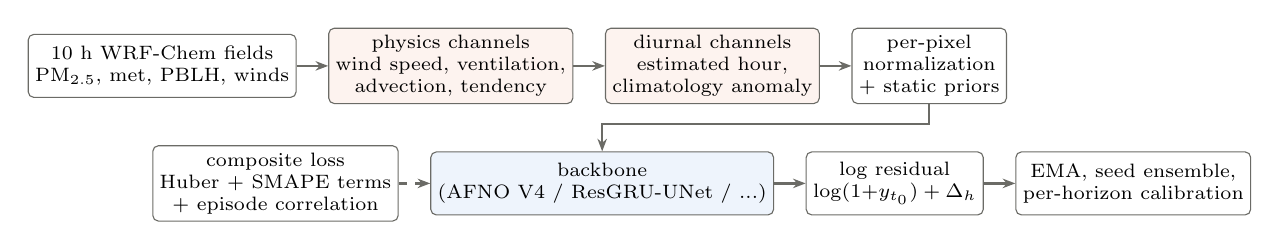
\begin{tikzpicture}[font=\scriptsize, node distance=3mm and 4mm,
  box/.style={draw=cgray, rounded corners=2pt, align=center, minimum height=8mm, inner sep=2.5pt, fill=white},
  phys/.style={box, fill=cafno!8},
  net/.style={box, fill=cres!8},
  arr/.style={-{Stealth[length=1.6mm]}, cgray, thick}]
\node[box] (raw) {10 h WRF-Chem fields\\ \PM, met, PBLH, winds};
\node[phys, right=of raw] (phys) {physics channels\\ wind speed, ventilation,\\ advection, tendency};
\node[phys, right=of phys] (time) {diurnal channels\\ estimated hour,\\ climatology anomaly};
\node[box, right=of time] (norm) {per-pixel\\ normalization\\ + static priors};
\node[net, below=6mm of time, xshift=-14mm] (bb) {backbone\\ (AFNO V4 / ResGRU-UNet / ...)};
\node[box, right=of bb] (res) {log residual\\ $\log(1{+}y_{t_0})+\Delta_h$};
\node[box, right=of res] (post) {EMA, seed ensemble,\\ per-horizon calibration};
\node[box, left=of bb] (loss) {composite loss\\ Huber + SMAPE terms\\ + episode correlation};
\draw[arr] (raw) -- (phys);
\draw[arr] (phys) -- (time);
\draw[arr] (time) -- (norm);
\draw[arr] (norm.south) |- ++(0,-2.5mm) -| (bb.north);
\draw[arr] (bb) -- (res);
\draw[arr] (res) -- (post);
\draw[arr, dashed] (loss) -- (bb);
\end{tikzpicture}

\vspace{6pt}
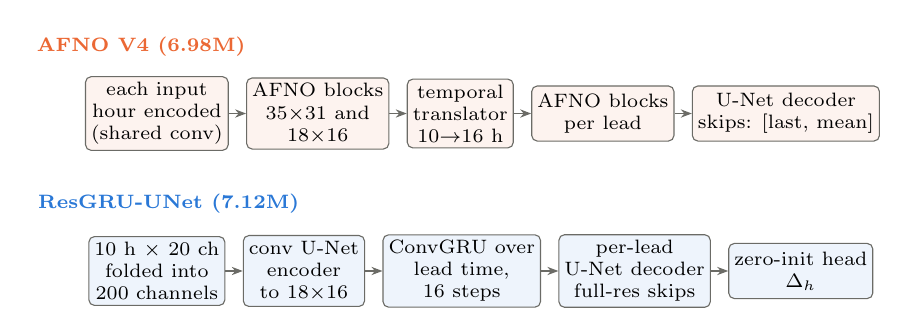
\begin{tikzpicture}[font=\scriptsize, node distance=2.2mm,
  b/.style={draw=cgray, rounded corners=2pt, align=center, minimum height=7mm, inner sep=2pt},
  arr/.style={-{Stealth[length=1.4mm]}, cgray}]
\node[font=\scriptsize\bfseries, text=cafno] at (-0.2,0.85) {AFNO V4 (6.98M)};
\node[b, fill=cafno!8] (a1) at (0,0) {each input\\ hour encoded\\ (shared conv)};
\node[b, fill=cafno!8, right=of a1] (a2) {AFNO blocks\\ 35$\times$31 and\\ 18$\times$16};
\node[b, fill=cafno!8, right=of a2] (a3) {temporal\\ translator\\ 10$\to$16 h};
\node[b, fill=cafno!8, right=of a3] (a4) {AFNO blocks\\ per lead};
\node[b, fill=cafno!8, right=of a4] (a5) {U-Net decoder\\ skips: [last, mean]};
\foreach \i/\j in {a1/a2,a2/a3,a3/a4,a4/a5} \draw[arr] (\i)--(\j);
\node[font=\scriptsize\bfseries, text=cres] at (0.15,-1.15) {ResGRU-UNet (7.12M)};
\node[b, fill=cres!8] (r1) at (0,-2.0) {10 h $\times$ 20 ch\\ folded into\\ 200 channels};
\node[b, fill=cres!8, right=of r1] (r2) {conv U-Net\\ encoder\\ to 18$\times$16};
\node[b, fill=cres!8, right=of r2] (r3) {ConvGRU over\\ lead time,\\ 16 steps};
\node[b, fill=cres!8, right=of r3] (r4) {per-lead\\ U-Net decoder\\ full-res skips};
\node[b, fill=cres!8, right=of r4] (r5) {zero-init head\\ $\Delta_h$};
\foreach \i/\j in {r1/r2,r2/r3,r3/r4,r4/r5} \draw[arr] (\i)--(\j);
\end{tikzpicture}
\caption{Top: the forecasting pipeline shared by all models. Physics and diurnal channels (orange) are computed from the input window; the backbone (blue) predicts a log-space change from the last input hour. Bottom: the two finalist backbones. AFNO V4 encodes each hour separately and mixes the sequence in a coarse spectral bottleneck; ResGRU-UNet stacks all hours as channels from the first convolution and unrolls a ConvGRU over lead time.}
\label{fig:pipeline}
\end{figure}

Figure~\ref{fig:pipeline} summarizes the pipeline. Every element below was added for a stated physical or statistical reason and kept only when it helped on a leak-free validation.

\subsection{Physics-informed inputs}
\label{sec:physics}
Surface \PM{} is governed by emission, transport, vertical mixing, chemistry and deposition. Three of these processes leave a signature in the available fields, and we encode each one explicitly rather than leaving the network to discover it from raw variables.

\paragraph{Vertical mixing: ventilation}
The boundary layer dilutes surface pollution in proportion to its depth and the horizontal wind that flushes it. Their product, the ventilation coefficient, is a standard indicator of pollution potential; its long-term decline over Indian cities is associated with increasing pollution potential \citep{iyer2013}. We add $V=\log\!\big(1+\mathrm{PBLH}\cdot\|\mathbf{u}_{10}\|\big)$ and the wind speed $\|\mathbf{u}_{10}\|$ as channels. Stagnation (low $V$) is when episodes build up.

\paragraph{Horizontal transport: advection}
To first order, a tracer follows $\partial_t C=-\mathbf{u}\cdot\nabla C$. We add the advection tendency of the log concentration, $A=-(u\,\partial_x+v\,\partial_y)\log(1+C)$, computed with centred differences on the grid. The scale matters: the mean 10-m wind over the training region is 4.24\,m\,s$^{-1}$, so \PM{} travels about 10 cells (244\,km) in 16 hours. A forecaster therefore needs a receptive field of roughly 10--12 cells in the horizontal, but no global one. One of the earlier models (ConvLSTM) applied this idea as a parameter-free semi-Lagrangian shift of the \PM{} frame along the wind \citep{staniforth1991}. FMG-WACLU added wind speed, direction and divergence, where convergence ($\nabla\cdot\mathbf{u}<0$) traps pollutants.

\paragraph{Temporal state: tendency and diurnal cycle}
A window-local tendency $\Delta_t\log(1+C)$, scaled by its per-cell standard deviation, separates building from decaying episodes. \PM{} has a strong diurnal cycle tied to the boundary layer. The test windows carry no timestamps, so we estimate each window's start hour by matching its mean shortwave radiation and temperature to hourly templates from training. This is correct within one hour for 97.7\% of validation windows, and validation uses the same estimate as the test, so it sees the same noise. The hour is encoded as $(\sin,\cos)$, together with the deviation of $\log(1+C)$ from the cell's hourly climatology. That deviation mirrors the STL residual that defines an episode.

\paragraph{Static priors and normalization}
Latitude, longitude, the per-cell \PM{} climatology and the per-cell STL residual spread are added as four static channels, for 20 channels in total. \PM{} and rain are log-transformed, and every channel is standardized per cell using training-period statistics, with a floor on the standard deviation and clipping at $\pm10$.

\subsection{Output, loss and validation}

\paragraph{Log-space persistence residual}
Persistence is a strong forecast at short lead times, so every network predicts a change from it: $\hat y_h=\exp\!\big(\log(1+y_{t_0})+\Delta_h\big)-1$ with a zero-initialized output layer \citep{he2016}. At initialization each model is exactly persistence. Working in log space matches the SMAPE geometry and the heavy right tail of \PM.

\paragraph{Metric-aligned loss}
Training minimizes $0.40\,\mathrm{Huber}(\log)+0.25\,G+0.15\,E+0.20\,(1-\rho)$ with episode cells up-weighted by 6. Lead hours are weighted linearly from 0.7 to 1.3, because errors grow with lead time while the score averages all hours equally.

\paragraph{Leak-free validation}
Windows are 26 hours long. With a random split, almost every validation window has a training neighbour sharing 24 or 25 of its 26 hours, including most targets, so validation is optimistic \citep{roberts2017}. We hold out the last 18\% of each month, leave a 12-hour gap before it, and score 214 validation windows (stride 2) with the exact metric. The checkpoint is selected on that score rather than on the loss.

\paragraph{Post-processing}
Weights are averaged with an exponential moving average (decay 0.999) \citep{polyak1992}, seeds are ensembled \citep{lakshminarayanan2017}, and each lead hour is multiplied by a factor fitted on validation from a 21-point grid in $[0.90,1.10]$. Pearson correlation is scale-invariant, so calibration moves only the SMAPE terms. Episode cells are selected where the truth turned out high, which makes upward-shifted forecasts score better on the episode terms. The fitted factors indeed rise with lead time, from 1.00 to 1.08--1.10.

\paragraph{Training}
AdamW \citep{loshchilov2019} (learning rate $2.5\times10^{-4}$, weight decay $10^{-4}$), a one-cycle schedule \citep{smith2019}, 16 epochs, an effective batch of 4, mixed precision and gradient clipping at 1.0. Normalization layers are GroupNorm \citep{wu2018}. One run takes about 51 minutes (ResGRU-UNet) or 90 minutes (AFNO V4) on a single NVIDIA T4.

% ================================================================
\section{How the pipeline was developed}
\label{sec:pipeline}

\begin{figure}[t]
\centering
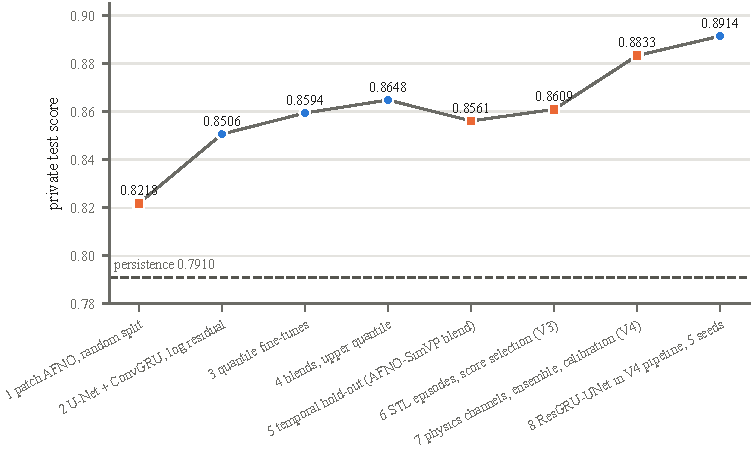
\includegraphics[width=\linewidth]{figures/fig_pipeline_evolution.pdf}
\caption{Held-out test score of the best model at each development iteration. Orange squares: AFNO family; blue circles: convolutional-recurrent family. The dashed line is persistence (0.7910). Iteration 5 rebuilt the pipeline on an honest temporal split and scored below iteration 4; the rebuilt pipeline overtakes it from iteration 6.}
\label{fig:evolution}
\end{figure}

\begin{table}[t]
\caption{Development iterations, what changed and why. Test scores are from the held-out test set.}
\label{tab:iterations}
\centering\small
\begin{tabular}{@{}c >{\raggedright\arraybackslash}p{5.6cm} >{\raggedright\arraybackslash}p{5.4cm} c@{}}
\toprule
\# & change & motivation & test \\
\midrule
1 & patch AFNO (4$\times$4 patches), random split & spectral mixing as in FourCastNet & 0.8218 \\
2 & U-Net + ConvGRU, log-space persistence residual, log Huber loss & persistence is strong; predict the change in log space & 0.8506 \\
3 & fine-tunes with asymmetric episode loss and pinball loss ($q{=}0.75$) \citep{koenker1978} & peaks were under-predicted & 0.8594 \\
4 & blends with upper-quantile models ($q{=}0.85$--$0.90$) & shift toward episode peaks & 0.8648 \\
5 & temporal hold-out; AFNO + SimVP translator, blended & the random split leaked targets & 0.8561 \\
6 & official STL episodes, 12-h gap, score-based selection, hour estimation (V3) & validation must match the metric and test & 0.8609 \\
7 & physics channels, multiscale AFNO block, horizon weights, 2 seeds, calibration (V4) & transport and mixing; long-lead errors & 0.8833 \\
8 & ResGRU-UNet trained in the V4 pipeline, 5 seeds, calibration & controlled backbone study & 0.8914 \\
\bottomrule
\end{tabular}
\end{table}

Table~\ref{tab:iterations} and Figure~\ref{fig:evolution} trace the eight iterations.

Iterations 1--4 used random validation splits, so their validation scores were inflated. The jump from 1 to 2 came with three simultaneous changes: a persistence residual, U-Net skips and a log-space Huber loss. Iterations 3 and 4 shifted the forecast toward high quantiles. This helps the episode terms but, under SMAPE, costs on the 98\% of cells that are background: the median is optimal for the global term. Zero-shot "physics multipliers" that scaled predictions under stagnation were tried in this phase and lost 0.006 for the same reason.

Iteration 5 introduced the temporal hold-out. Iteration 6 (V3) made validation reproduce the metric and the test conditions:
\begin{itemize}[leftmargin=14pt]
\item official STL episodes
\item a gap before the validation block
\item checkpoint selection on the score
\item hour estimation, which fixed a train/test mismatch in the hour features
\end{itemize}

Iteration 7 (V4) added the physics channels of Section~\ref{sec:physics}, one AFNO block at intermediate resolution and horizon weights, then a 2-seed ensemble and calibration. Its +0.0224 test gain over V3 splits into +0.0147 from the per-seed model changes, +0.0024 from ensembling and +0.0054 from calibration. On validation, V4 adds +0.060 over persistence.

% ================================================================
\section{Controlled backbone study}
\label{sec:study}

\paragraph{Protocol}
Five architectures were retrained inside the V4 pipeline (Table~\ref{tab:round1}). The inputs, split, episode masks, loss, recipe and 214 validation windows are identical; only the network differs. With the original input width and the same weights, each port reproduces its original network's output exactly (ConvLSTM's season conditioning, which has no input here, was removed). A bug in the original patch AFNO, which discarded the imaginary part of every filtered spectrum, was fixed. Before each stage, a decision rule was written down. A model is called better only if it leads by more than 0.003 on validation and also scores higher on the held-out test; otherwise the result is a tie or inconclusive. The study ran in three stages: one seed for all five networks; the two finalists with two seeds and the full V4 recipe; then five seeds per finalist.

\begin{table}[t]
\caption{Round one: one seed (42), identical pipeline, no ensembling or calibration. Validation uses equal metric weights.}
\label{tab:round1}
\centering\small
\begin{tabular}{@{}l l r c c@{}}
\toprule
model & design & params & val score & test score \\
\midrule
ResGRU-UNet & U-Net + ConvGRU over lead time & 7.12M & \textbf{0.9158} & \textbf{0.8798} \\
AFNO V4 & per-hour encoder, AFNO blocks, translator & 6.98M & 0.9110 & 0.8762 \\
FMG-WACLU & ConvLSTM U-Net, wind physics, future-met gate & 3.45M & 0.9099 & 0.8710 \\
patch AFNO & 4$\times$4 patches, AFNO, linear unpatchify & 5.71M & 0.9031 & 0.8530 \\
ConvLSTM & ConvLSTM over inputs, spectral block, advection shift & 19.0M & 0.8945 & 0.8452 \\
\bottomrule
\end{tabular}
\end{table}

\paragraph{Round one}
ResGRU-UNet leads on validation and test (Table~\ref{tab:round1}). Validation and test order the five models identically, which supports the validation design. ResGRU-UNet beats AFNO V4 under the rule (+0.0048 validation, +0.0036 test). FMG-WACLU ties with AFNO V4 on validation, and patch AFNO and ConvLSTM are worse.

\paragraph{Final round and five seeds}
With two seeds, an ensemble and calibration for both finalists, ResGRU-UNet again leads: 0.9175 vs 0.9131 on validation, and 0.8898 vs 0.8833 on test. Three more seeds per finalist give the results in Table~\ref{tab:fiveseed} and Figure~\ref{fig:seeds}. The gap between the 5-seed ensembles is +0.00479 on validation, with a 95\% block-bootstrap interval of [+0.00383, +0.00578]: blocks of 13 consecutive windows within each month, 2{,}000 resamples. Every ResGRU-UNet seed beats every AFNO V4 seed on validation and on test (25 of 25 pairs). The worst ResGRU-UNet seed (0.8788 test) beats the best AFNO V4 seed (0.8767).

\begin{table}[t]
\caption{Five seeds per finalist. Validation scores use equal metric weights; test scores are from the held-out test set. Calibration is fitted on validation.}
\label{tab:fiveseed}
\centering\small
\begin{tabular}{@{}l c c c@{}}
\toprule
 & AFNO V4 & ResGRU-UNet & gap \\
\midrule
single seeds, val (mean $\pm$ sd) & 0.91146 $\pm$ 0.00059 & 0.91630 $\pm$ 0.00104 & +0.00484 \\
5-seed ensemble, val & 0.91454 & 0.91933 & +0.00479 \\
\quad + calibration (leave-one-month-out) & 0.91492 & 0.92097 & +0.00605 \\
single seeds, test (mean $\pm$ sd) & 0.87540 $\pm$ 0.00130 & 0.87994 $\pm$ 0.00085 & +0.00454 \\
5-seed ensemble, test & 0.8793 & 0.8838 & +0.0045 \\
\quad + calibration, test & 0.8848 & \textbf{0.8914} & +0.0066 \\
\bottomrule
\end{tabular}
\end{table}

\begin{figure}[t]
\centering
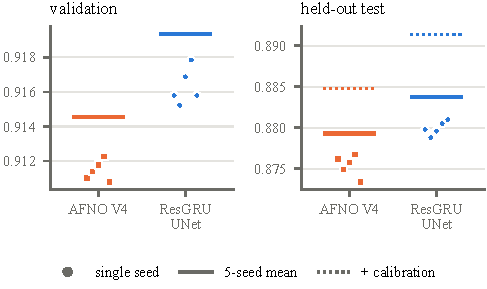
\includegraphics[width=\linewidth]{figures/fig_seed_spread.pdf}
\caption{Seed spread. Markers are single seeds; solid lines are 5-seed ensembles and dotted lines the calibrated ensembles. The two families do not overlap on validation or on the held-out test.}
\label{fig:seeds}
\end{figure}

\paragraph{Pipeline versus backbone}
Moving ResGRU-UNet from its iteration-2 setup into the V4 pipeline raised its test score from 0.8506 to 0.8798 (+0.0292, one seed, no calibration). At that same setting the backbone gap to AFNO V4 is +0.0036, or +0.0045 averaged over five single seeds. The pipeline therefore moved the score 6 to 8 times more than the choice between the two best networks (4.4 times against the full-recipe gap of +0.0066). The pipeline gain is one bundle of changes: inputs, split and checkpoint selection, hour estimation, episode masks, loss, schedule and EMA. We did not isolate its parts.

% ================================================================
\section{Analysis}
\label{sec:analysis}

\paragraph{Regression metrics}
Table~\ref{tab:regression} reports MAE, RMSE and $R^2$ on validation for every model and baseline. The ridge baseline is a single linear model shared by all cells. It takes the 20 channels at the last input hour plus log \PM{} at the nine earlier hours, predicts the 16 log-space changes, and is fitted in closed form \citep{hoerl1970} on 2.45 million training cell-windows, with the penalty chosen on validation. Ridge improves on persistence on validation (score 0.8637 vs 0.8515), but on the test set it barely does (0.7951 vs 0.7910). Every network beats all three baselines on every metric. ResGRU-UNet's 5-seed ensemble reduces MAE by 39\% and RMSE by 32\% relative to persistence. The seasonal-naive forecast is worse than persistence overall but better from lead hour 8 on (Figure~\ref{fig:lead}), because the diurnal cycle eventually dominates the last observed state.

\begin{table}[t]
\caption{Validation regression metrics ($\mu$g\,m$^{-3}$ for MAE and RMSE), pooled over all $5.9\times10^7$ values, with the benchmark score (equal weights). The uncalibrated ensembles are best on MAE, RMSE and $R^2$; calibration helps only the score.}
\label{tab:regression}
\centering\small
\begin{tabular}{@{}l c c c c c@{}}
\toprule
model & MAE & RMSE & $R^2$ & $R^2$ (log) & score \\
\midrule
persistence & 10.44 & 26.46 & 0.767 & 0.895 & 0.8515 \\
seasonal naive (24 h earlier) & 11.53 & 26.80 & 0.761 & 0.832 & 0.7907 \\
ridge regression & 8.51 & 21.48 & 0.847 & 0.923 & 0.8637 \\
\midrule
patch AFNO (seed 42) & 6.85 & 19.02 & 0.880 & 0.943 & 0.9031 \\
ConvLSTM (seed 42) & 7.05 & 18.93 & 0.881 & 0.940 & 0.8945 \\
FMG-WACLU (seed 42) & 7.14 & 19.32 & 0.876 & 0.942 & 0.9099 \\
AFNO V4 (seed 42) & 7.31 & 20.17 & 0.865 & 0.941 & 0.9110 \\
ResGRU-UNet (seed 42) & 6.57 & 18.57 & 0.885 & 0.949 & 0.9158 \\
\midrule
AFNO V4, 5-seed ensemble & 6.99 & 19.45 & 0.874 & 0.944 & 0.9145 \\
\quad + calibration (leave-one-month-out) & 7.76 & 20.90 & 0.855 & 0.938 & 0.9149 \\
ResGRU-UNet, 5-seed ensemble & \textbf{6.32} & \textbf{18.04} & \textbf{0.892} & \textbf{0.952} & 0.9193 \\
\quad + calibration (leave-one-month-out) & 7.12 & 19.71 & 0.871 & 0.946 & \textbf{0.9210} \\
\bottomrule
\end{tabular}
\end{table}

\begin{figure}[t]
\centering
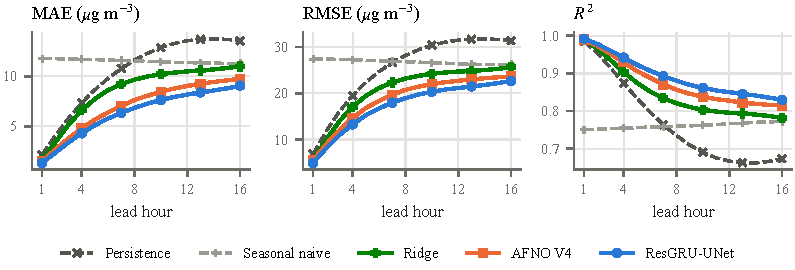
\includegraphics[width=\linewidth]{figures/fig_lead_metrics.pdf}
\caption{Validation MAE, RMSE and $R^2$ per lead hour for the baselines and the two finalists (5-seed ensembles, uncalibrated). ResGRU-UNet is best at every lead hour.}
\label{fig:lead}
\end{figure}

\paragraph{Rankings depend on the metric}
ResGRU-UNet ranks first on all six measures in Figure~\ref{fig:rank}. The other four architectures reorder: AFNO V4 is second on the benchmark score but last on MAE, RMSE and $R^2$, while ConvLSTM is last on the score but second on RMSE and $R^2$. The benchmark score is relative and focused on episodes, whereas MAE, RMSE and raw-scale $R^2$ are dominated by high concentrations. A single metric would therefore have given a misleading picture of the weaker architectures.

\begin{figure}[t]
\centering
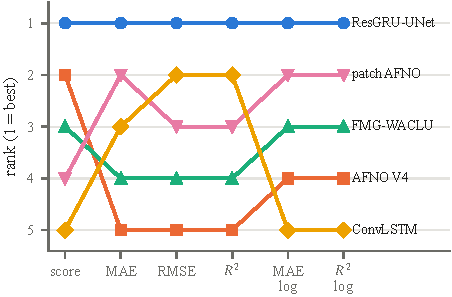
\includegraphics[width=0.95\linewidth]{figures/fig_rank_by_metric.pdf}
\caption{Round-one ranks (seed 42) of the five architectures under six measures. Only the winner is stable.}
\label{fig:rank}
\end{figure}

\paragraph{Calibration trades error for score}
Per-horizon calibration raises the benchmark score but increases MAE and RMSE and lowers $R^2$ for both finalists (Figure~\ref{fig:calib}). For example, the ResGRU-UNet ensemble moves from MAE 6.32 to 7.12 while its validation score rises from 0.9193 to 0.9210. The factors push predictions up. This is rewarded by the SMAPE terms through the episode selection effect, but penalized by absolute and squared errors. Which version to deploy therefore depends on the objective.

\begin{figure}[t]
\centering
\begin{minipage}[t]{0.58\linewidth}\vspace{0pt}
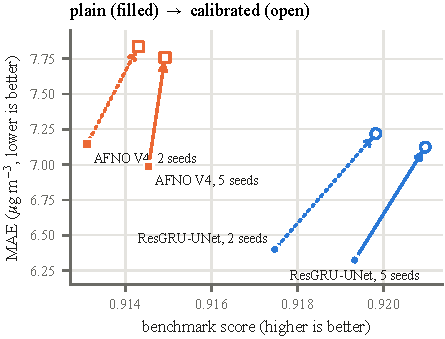
\includegraphics[width=\linewidth]{figures/fig_calibration.pdf}
\end{minipage}\hfill
\begin{minipage}[t]{0.39\linewidth}\vspace{4pt}
\caption{Calibration moves both finalists to a higher benchmark score (right) but a larger MAE (up). Filled: uncalibrated ensembles; open: calibrated, in sample for 2 seeds and leave-one-month-out for 5 seeds.}
\label{fig:calib}
\end{minipage}
\end{figure}

\paragraph{Where ResGRU-UNet wins}
The validation gap grows from +0.0018 at hour 1 to about +0.006 at hours 10--15, and ResGRU-UNet is better on all three metric terms at every hour. Of the score gap, 56\% comes from the global SMAPE term, 23\% from episode SMAPE and 22\% from episode correlation. It is ahead in all four validation months and in five of six concentration bins (Figure~\ref{fig:where}), and has the lower mean SMAPE in 94.7\% of grid cells. Both models under-predict episode cells by a similar amount (mean log bias $-0.160$ and $-0.157$) and over-predict the remaining cells ($+0.084$ and $+0.062$). ResGRU-UNet's smaller over-prediction outside episodes is consistent with its larger gain in the global term.

\begin{figure}[t]
\centering
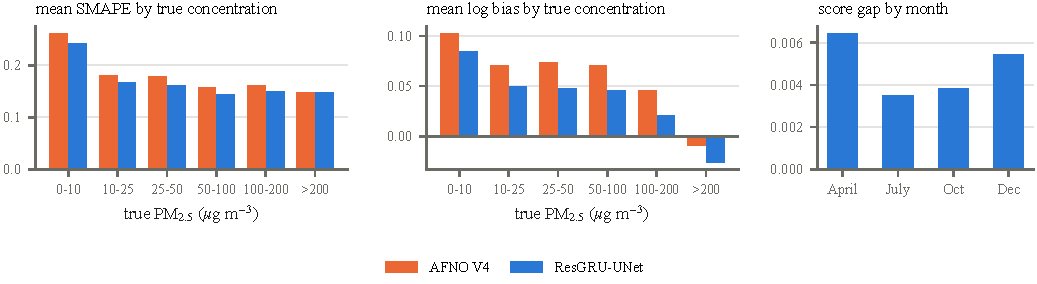
\includegraphics[width=\linewidth]{figures/fig_where.pdf}
\caption{Left: mean SMAPE by true concentration for the 5-seed ensembles. Right: validation score gap by month.}
\label{fig:where}
\end{figure}

\paragraph{Spatial structure}
Figure~\ref{fig:maps} maps the time-averaged errors. Concentrations and errors concentrate in the Indo-Gangetic Plain, where persistence errors are largest. ResGRU-UNet removes much of that error. It has the lower MAE than AFNO V4 in 90.5\% of cells, with the largest reductions over the Indo-Gangetic Plain and central India, so its advantage is not confined to one region. The median per-cell $R^2$ over time is 0.872 for ResGRU-UNet, 0.846 for AFNO V4 and 0.694 for persistence. It is lowest north of 32$^\circ$N (median 0.764), where concentrations are lowest (13.8 vs 42.3\,$\mu$g\,m$^{-3}$ south of it). A case study of the window with the most episode cells is in Appendix~\ref{app:case}.

\IfFileExists{figures/fig_maps.pdf}{
\begin{figure}[t]
\centering
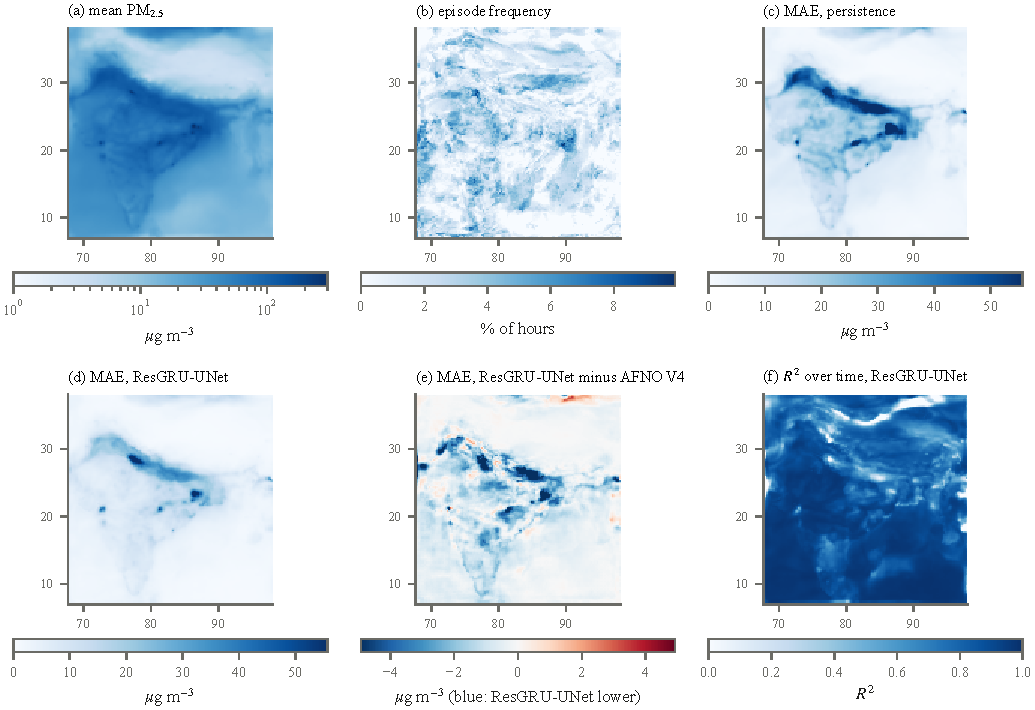
\includegraphics[width=\linewidth]{figures/fig_maps.pdf}
\caption{Time-averaged validation maps. (a) Mean \PM. (b) Episode frequency. (c, d) MAE of persistence and of the ResGRU-UNet ensemble. (e) MAE difference, ResGRU-UNet minus AFNO V4 (blue: ResGRU-UNet lower). (f) Per-cell $R^2$ over time for ResGRU-UNet.}
\label{fig:maps}
\end{figure}}{}

\paragraph{Cost}
ResGRU-UNet is also cheaper: 25.8 vs 48.6\,ms per window at inference, 0.23 vs 1.36\,GB of peak inference memory at batch size 4, and 191 vs 338\,s per training epoch on a T4.

% ================================================================
\section{Why does the convolutional-recurrent model win?}
\label{sec:why}

\paragraph{Ablations}
We tested four hypotheses, each with one change to one finalist and one seed (Table~\ref{tab:ablations}). The predictions and the decision rule were written down before the runs. A change counts as resolved only if it moves validation by more than $\max(2\,\mathrm{sd},0.002)$ from its family's 5-seed mean.
\begin{itemize}[leftmargin=14pt]
\item H1: AFNO V4's skips keep only the last hour and the mean.
\item H2: the unpadded FFT wraps opposite edges of a non-periodic domain.
\item H3: soft-thresholding removes low-amplitude detail.
\item H4: ResGRU-UNet's recurrence over lead time is what makes it win.
\end{itemize}
None is resolved at one seed. H1 (all-hour skips, initialized to equal V4's fusion) is the largest move toward ResGRU-UNet, about a quarter of the gap. Replacing ResGRU-UNet's ConvGRU with per-lead convolutional blocks of equal size costs about a third of the gap, yet the model still beats every AFNO V4 seed. So the recurrence is not needed to win, but its share of the gap is unresolved. Padding the spectral blocks also strengthens their sparsity, because the orthonormal FFT spreads the same energy over four times as many coefficients; H3 suggests that effect is small.

\begin{table}[t]
\caption{Single-change ablations (seed 42). $d$: validation change from the family's 5-seed mean; $d/G$: share of the 0.00484 gap between the families. None exceeds the threshold of 0.002.}
\label{tab:ablations}
\centering\small
\begin{tabular}{@{}l l c c c c@{}}
\toprule
 & change & val & $d$ & $d/G$ & test \\
\midrule
H1 & AFNO V4, skips fuse all 10 hours & 0.91259 & +0.00113 & +0.23 & 0.8748 \\
H2 & AFNO V4, zero-padded spectral blocks & 0.91062 & $-$0.00084 & $-$0.17 & 0.8745 \\
H3 & AFNO V4, no soft-threshold & 0.91094 & $-$0.00052 & $-$0.11 & 0.8758 \\
H4 & ResGRU-UNet, ConvGRU replaced & 0.91456 & $-$0.00174 & $-$0.36 & 0.8798 \\
\bottomrule
\end{tabular}
\end{table}

\paragraph{A generalization gap}
The training curves show a pattern that none of the AFNO changes altered (Figure~\ref{fig:curves}). All AFNO runs reach a lower training loss than ResGRU-UNet but a higher validation loss: at a training loss of 0.09, AFNO's validation loss is 6.8\% higher on average. Its validation score peaks at epoch 4--5 and then drops by 0.009--0.010; ResGRU-UNet peaks at epoch 6--7 and drops by 0.003--0.005. Without its recurrence, ResGRU-UNet moves about 41\% of the way toward AFNO's validation loss. These are exploratory observations. They suggest that the Fourier model fits the training months more and transfers less to held-out months, but we have not isolated a cause. The global, periodic spectral mixing, the per-hour shared encoder and the temporal translator remain candidates. Physical scale is consistent with this reading: transport covers about 10 cells in 16 hours, so AFNO's global receptive field brings no needed information but adds capacity to fit month-specific large-scale patterns.

\begin{figure}[t]
\centering
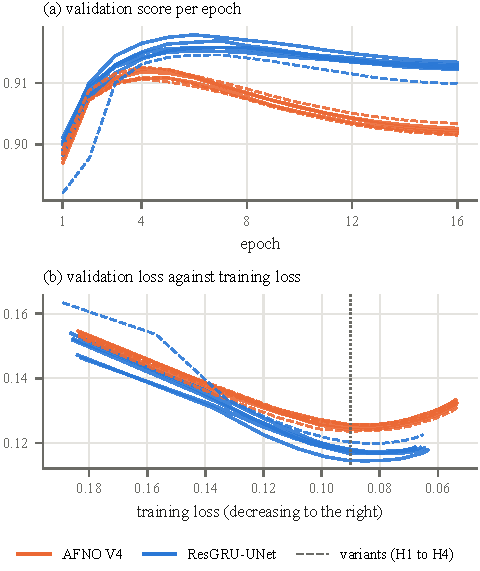
\includegraphics[width=\linewidth]{figures/fig_training_curves.pdf}
\caption{Training curves of all 12 logged runs. Left: validation score per epoch. Right: validation loss against training loss (training loss decreases to the right); the dotted line marks a training loss of 0.09.}
\label{fig:curves}
\end{figure}

% ================================================================
\section{Limitations}

\begin{itemize}[leftmargin=14pt]
\item \textbf{Data:} the data are simulations, not observations; skill on WRF-Chem fields need not transfer to monitored \PM.
\item \textbf{Evaluation sets:} there is one validation period (the tail of four months) and one test set. Validation chose each run's best epoch and fitted the calibration, so validation scores are optimistic for every model; the held-out test is the only untouched measure.
\item \textbf{Metric:} the metric's weights are undisclosed. We assume equal weights on validation, which may differ from the test scorer.
\item \textbf{Recipe:} the training recipe was tuned for AFNO V4, which if anything favours it. ResGRU-UNet received no tuning.
\item \textbf{Timing of the rules:} the decision rules were fixed before each stage, but the final rounds were designed after round one's result was known (2 of 5 seeds were already known).
\item \textbf{Statistics:} adjacent bootstrap blocks overlap in time, so the intervals may be narrow; the ablations use one seed each.
\item \textbf{Pipeline gain:} the pipeline gain bundles several changes that we did not isolate.
\end{itemize}

% ================================================================
\section{Conclusion}

For 16-hour \PM{} forecasting over India from WRF-Chem fields, the forecasting pipeline mattered more than the backbone. Physically motivated channels, a log-space persistence residual, leak-free validation that mirrors the test, a metric-aligned loss, and ensembling with calibration gave the same network a gain 6 to 8 times larger than the gap between the two best networks. Within one fixed pipeline, a simple convolutional-recurrent U-Net was consistently better than an AFNO hybrid: on every seed pair, lead hour, month and regression metric. It was also cheaper. Its advantage is not explained by any single component we tested. The Fourier model generalizes less well across months, which fits the local, non-periodic physics of a 16-hour transport problem. We recommend that architecture comparisons for air-quality emulation fix the pipeline first, report several metrics and seeds, and include persistence, seasonal-naive and linear baselines.

\paragraph{Code} The study code, notebooks and analysis scripts are available at \url{https://github.com/Vetri-78640/dl_pm2.5}.

% ================================================================
\small
\begin{thebibliography}{30}\setlength{\itemsep}{1pt}

\bibitem{aisehack2026} ANRF AISEHack 2026, Phase 2, Theme 2: pollution forecasting (IIT Delhi). Kaggle competition, 2026. \url{https://www.kaggle.com/competitions/anrf-aise-hack-phase-2-theme-2-pollution-forecasting-iitd}.

\bibitem{ballas2016convgru} N.~Ballas, L.~Yao, C.~Pal, and A.~Courville. Delving deeper into convolutional networks for learning video representations. In \emph{ICLR}, 2016.

\bibitem{bedi2025conoair} S.~Bedi, K.~Tiwari, Prathosh A.~P., S.~H.~Kota, N.~M.~A.~Krishnan, et al. CoNOAir: A neural operator for forecasting carbon monoxide evolution in cities. arXiv:2501.06007, 2025.

\bibitem{cleveland1990} R.~B.~Cleveland, W.~S.~Cleveland, J.~E.~McRae, and I.~Terpenning. STL: A seasonal-trend decomposition procedure based on loess. \emph{Journal of Official Statistics}, 6(1):3--73, 1990.

\bibitem{dang2025adaptfno} H.~V.~Dang, B.~D.~G.~Nguyen, P.~C.~H.~Nguyen, and T.-S.~Hy. AdaptFNO: Adaptive Fourier neural operator with dynamic spectral modes and multiscale learning for climate modeling. NeurIPS 2025 Workshop on Machine Learning and the Physical Sciences, 2025.

\bibitem{gao2022simvp} Z.~Gao, C.~Tan, L.~Wu, and S.~Z.~Li. SimVP: Simpler yet better video prediction. In \emph{CVPR}, pages 3170--3180, 2022.

\bibitem{goodwin1999} P.~Goodwin and R.~Lawton. On the asymmetry of the symmetric MAPE. \emph{International Journal of Forecasting}, 15(4):405--408, 1999.

\bibitem{grell2005} G.~A.~Grell, S.~E.~Peckham, R.~Schmitz, S.~A.~McKeen, G.~Frost, W.~C.~Skamarock, and B.~Eder. Fully coupled ``online'' chemistry within the WRF model. \emph{Atmospheric Environment}, 39(37):6957--6975, 2005.

\bibitem{guibas2022afno} J.~Guibas, M.~Mardani, Z.~Li, A.~Tao, A.~Anandkumar, and B.~Catanzaro. Efficient token mixing for transformers via adaptive Fourier neural operators. In \emph{ICLR}, 2022. arXiv:2111.13587.

\bibitem{he2016} K.~He, X.~Zhang, S.~Ren, and J.~Sun. Deep residual learning for image recognition. In \emph{CVPR}, pages 770--778, 2016.

\bibitem{hoerl1970} A.~E.~Hoerl and R.~W.~Kennard. Ridge regression: Biased estimation for nonorthogonal problems. \emph{Technometrics}, 12(1):55--67, 1970.

\bibitem{hyndman2021} R.~J.~Hyndman and G.~Athanasopoulos. \emph{Forecasting: Principles and Practice}. OTexts, 3rd edition, 2021.

\bibitem{iyer2013} U.~S.~Iyer and P.~E.~Raj. Ventilation coefficient trends in the recent decades over four major Indian metropolitan cities. \emph{Journal of Earth System Science}, 122(2):537--549, 2013.

\bibitem{koenker1978} R.~Koenker and G.~Bassett Jr. Regression quantiles. \emph{Econometrica}, 46(1):33--50, 1978.

\bibitem{kushwaha2025} A.~Kushwaha and K.~Gopalan. A comparison of lightweight deep learning models for particulate-matter nowcasting in the Indian subcontinent \& surrounding regions. arXiv:2511.11185, 2025.

\bibitem{lakshminarayanan2017} B.~Lakshminarayanan, A.~Pritzel, and C.~Blundell. Simple and scalable predictive uncertainty estimation using deep ensembles. In \emph{NeurIPS}, pages 6402--6413, 2017.

\bibitem{leinonen2021} J.~Leinonen. Spatiotemporal weather data predictions with shortcut recurrent-convolutional networks: A solution for the Weather4cast challenge. arXiv:2111.02121, 2021.

\bibitem{li2021fno} Z.~Li, N.~Kovachki, K.~Azizzadenesheli, B.~Liu, K.~Bhattacharya, A.~Stuart, and A.~Anandkumar. Fourier neural operator for parametric partial differential equations. In \emph{ICLR}, 2021.

\bibitem{loshchilov2019} I.~Loshchilov and F.~Hutter. Decoupled weight decay regularization. In \emph{ICLR}, 2019.

\bibitem{pandey2021} A.~Pandey et al. (India State-Level Disease Burden Initiative Air Pollution Collaborators). Health and economic impact of air pollution in the states of India: the Global Burden of Disease Study 2019. \emph{The Lancet Planetary Health}, 5(1):e25--e38, 2021.

\bibitem{pathak2022fourcastnet} J.~Pathak, S.~Subramanian, P.~Harrington, S.~Raja, A.~Chattopadhyay, M.~Mardani, T.~Kurth, D.~Hall, Z.~Li, K.~Azizzadenesheli, et al. FourCastNet: A global data-driven high-resolution weather model using adaptive Fourier neural operators. arXiv:2202.11214, 2022.

\bibitem{polyak1992} B.~T.~Polyak and A.~B.~Juditsky. Acceleration of stochastic approximation by averaging. \emph{SIAM Journal on Control and Optimization}, 30(4):838--855, 1992.

\bibitem{roberts2017} D.~R.~Roberts, V.~Bahn, S.~Ciuti, M.~S.~Boyce, J.~Elith, G.~Guillera-Arroita, S.~Hauenstein, J.~J.~Lahoz-Monfort, B.~Schr\"oder, W.~Thuiller, D.~I.~Warton, B.~A.~Wintle, F.~Hartig, and C.~F.~Dormann. Cross-validation strategies for data with temporal, spatial, hierarchical, or phylogenetic structure. \emph{Ecography}, 40(8):913--929, 2017.

\bibitem{ronneberger2015unet} O.~Ronneberger, P.~Fischer, and T.~Brox. U-Net: Convolutional networks for biomedical image segmentation. In \emph{MICCAI}, pages 234--241, 2015.

\bibitem{shi2015convlstm} X.~Shi, Z.~Chen, H.~Wang, D.-Y.~Yeung, W.-k.~Wong, and W.-c.~Woo. Convolutional LSTM network: A machine learning approach for precipitation nowcasting. In \emph{NeurIPS}, pages 802--810, 2015.

\bibitem{shi2017trajgru} X.~Shi, Z.~Gao, L.~Lausen, H.~Wang, D.-Y.~Yeung, W.-k.~Wong, and W.-c.~Woo. Deep learning for precipitation nowcasting: A benchmark and a new model. In \emph{NeurIPS}, 2017.

\bibitem{smith2019} L.~N.~Smith and N.~Topin. Super-convergence: Very fast training of neural networks using large learning rates. In \emph{Proc. SPIE 11006}, 2019.

\bibitem{staniforth1991} A.~Staniforth and J.~C\^ot\'e. Semi-Lagrangian integration schemes for atmospheric models: A review. \emph{Monthly Weather Review}, 119(9):2206--2223, 1991.

\bibitem{wu2018} Y.~Wu and K.~He. Group normalization. In \emph{ECCV}, pages 3--19, 2018.

\end{thebibliography}
\normalsize

% ================================================================
\appendix
\section{Implementation details}
\label{app:impl}

\begin{table}[h]
\caption{Training and evaluation settings shared by all networks in the controlled study.}
\centering\small
\begin{tabular}{@{}l >{\raggedright\arraybackslash}p{10.2cm}@{}}
\toprule
input / output & 10 hours, 20 channels $\to$ 16 hours of \PM{} \\
split & last 18\% of each month for validation, 12-h gap; 2{,}257 train and 214 validation windows (stride 2) \\
loss & $0.40$ Huber($\log$) $+ 0.25\,G + 0.15\,E + 0.20(1-\rho)$, episode weight 6, horizon weights 0.7--1.3 \\
optimizer & AdamW, lr $2.5\times10^{-4}$, weight decay $10^{-4}$, one-cycle, 16 epochs, effective batch 4 \\
stabilization & EMA 0.999, mixed precision, gradient clipping 1.0, GroupNorm \\
selection & best epoch by the validation score (equal weights) \\
calibration & per lead hour, 21-point grid in $[0.90, 1.10]$ \\
bootstrap & blocks of 13 consecutive windows within a month, 2{,}000 resamples \\
hardware & one NVIDIA T4 per run \\
\bottomrule
\end{tabular}
\end{table}

\paragraph{Ridge baseline}
Features per cell are the 20 normalized channels at the last input hour, log \PM{} at the nine earlier hours and a bias (30 values). Targets are the 16 changes $\log(1+y_h)-\log(1+y_{t_0})$. We solve $W=(X^\top X+\lambda I')^{-1}X^\top Y$, with the bias unpenalized, on every fourth cell in each direction of all training windows, and choose $\lambda\in\{10^{-2},1,10^{2},10^{4},10^{6}\}$ on the validation score ($\lambda=10^{-2}$). With zero weights the model reproduces persistence exactly, which we verified.

\paragraph{Verification}
Every stage was dry-run on synthetic data before training, and every analysis cross-checks its numbers against the earlier runs. For example, the regression metrics recompute each model's benchmark score and match its logged value within $10^{-4}$, and persistence reproduces 0.8515.

\section{Case study}
\label{app:case}

\begin{figure}[h]
\centering
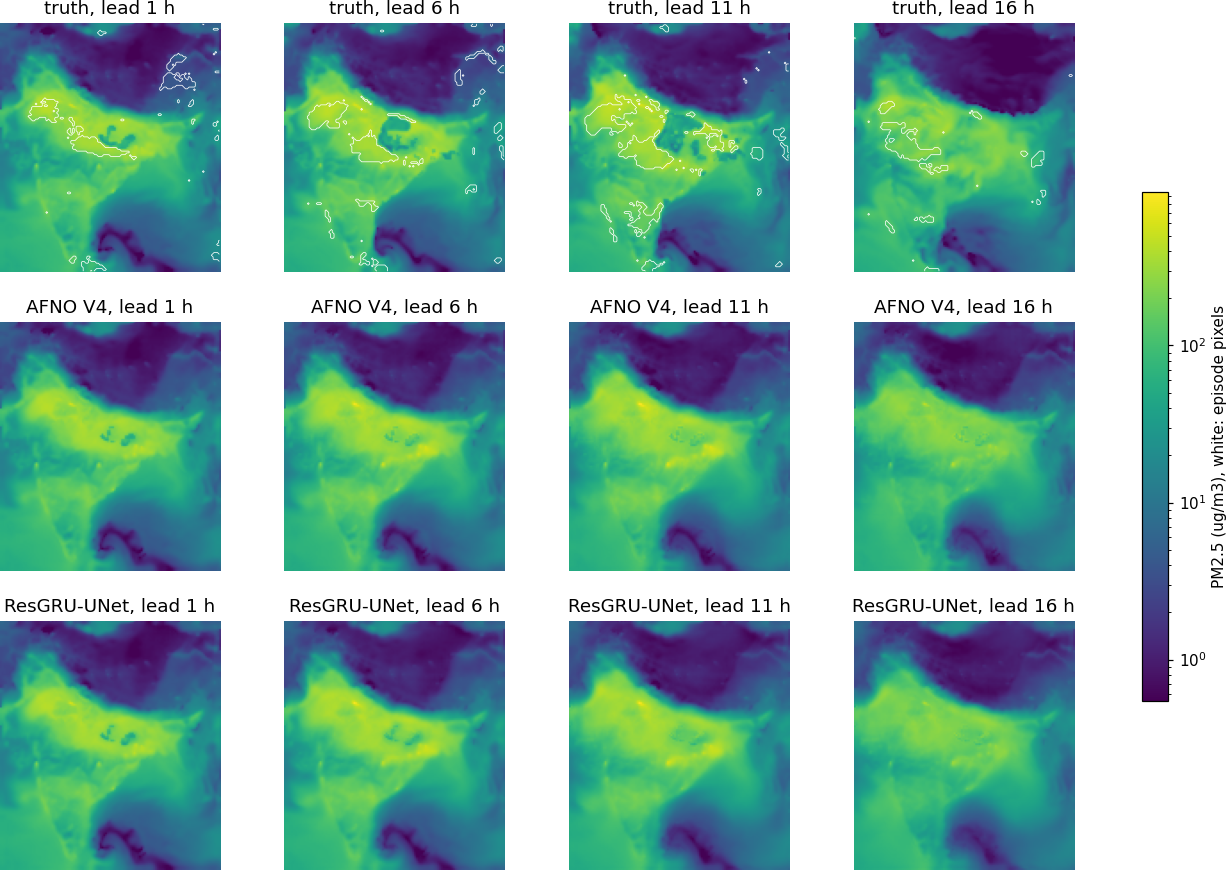
\includegraphics[width=\linewidth]{figures/fig_case.png}
\caption{The validation window with the most episode cells (December). Rows: truth with episode cells outlined, AFNO V4 ensemble, ResGRU-UNet ensemble, at lead hours 1, 6, 11 and 16 (grid coordinates, log colour scale). Both ensembles smooth the episode structure; ResGRU-UNet scores higher on this window (0.9116 vs 0.9103) but has a lower episode correlation (0.928 vs 0.944).}
\end{figure}

\section{Per-lead-hour validation metrics}

\begin{table}[h]
\caption{Validation MAE ($\mu$g\,m$^{-3}$) and $R^2$ at selected lead hours (5-seed ensembles, uncalibrated).}
\centering\small
\begin{tabular}{@{}l ccccc ccccc@{}}
\toprule
 & \multicolumn{5}{c}{MAE at lead hour} & \multicolumn{5}{c}{$R^2$ at lead hour} \\
\cmidrule(lr){2-6}\cmidrule(lr){7-11}
model & 1 & 4 & 8 & 12 & 16 & 1 & 4 & 8 & 12 & 16 \\
\midrule
persistence & 2.14 & 7.32 & 11.63 & 13.58 & 13.57 & 0.985 & 0.875 & 0.735 & 0.667 & 0.674 \\
AFNO V4 & 1.49 & 4.77 & 7.62 & 9.04 & 9.76 & 0.990 & 0.930 & 0.857 & 0.828 & 0.815 \\
ResGRU-UNet & 1.31 & 4.29 & 6.84 & 8.18 & 9.07 & 0.992 & 0.942 & 0.881 & 0.850 & 0.830 \\
\bottomrule
\end{tabular}
\end{table}

\end{document}
